\chapter{Data Visualization}

Data Visualization is the visual representation of data using plots and visual models. In the infrastructural stack stands at the highest level since it's the mean through which the result of all the processing is shown. The reason that makes it so important is that humans are not able to extract useful information from raw data at a glance, and thus comes the need for clear and intuitive plots capturing all the helpful statistics contained, in a concise way: insights from which human can act accordingly.

The stack uses as a visualization tool Tableau, and in this chapter will be presented its structure and its strengths. 

\section{Introduction}

Tableau is a software dedicated to creation of visualizations for the Business Intelligence. According to Gartner \cite{gartner_tableau}, Tableau offers an highly intuitive and interactive way to the access, manipulation and analysis of data, without the need for coding, positioning itself among the first three product leaders in the sector. Tableau's main features include easiness and intuitiveness in the software use, data sources management and some innovative features such as table calculations and the possibility to use data analysis techniques directly on the plots.

Tableau On Premise version is composed of two elements:

\begin{itemize}
    \item \textbf{Tableau Desktop}: Allows for the creation of worksheets, dashboards and stories, linked to one or more data sources.
    \item \textbf{Tableau Server}: It is used to publish the plots created with Tableau Desktop, in order to make them available to end users.
\end{itemize}

\section{Tableau Desktop}

Tableau is structured in a Microsoft Excel fashion, with workbooks and sheets: a workbook is made of many sheets which can be worksheets, dashboards or stories. A worksheet is a single plot, with its own filters and legend, and can be combined with other worksheets to make a dashboard. A story is a sequence of dashboards and it's usually the view shown to the end user. Each workbook starts from one or more data sources, used by Tableau for fetching the data used in the plots.

\subsection{Data Source}

The first step during the creation of a workbook is to link Tableau to a data source \cite{LearningTableau}, either through a \textbf{File Connection}, which supports all of the main data formats available such as JSON, CSV, TSV, PDF and Excel sheets, or a \textbf{Server Connection}, to relational databases, such as Microsoft SQL Server and Hive, NoSQL databases, such as MongoDB or Cassandra, and data sources in cloud, such as Google Analytics, Amazon Redshift and Salesforce. If there's no optimized built-in driver, it's possible to use any ODBC\footnote{ODBC: Open DataBase Connectivity is a standard API to access DBMS} driver. Any interaction with a data source is handled by default with \textbf{VizQL} (Visual Query Language), which translates all of the drag-n-drop actions executed in the GUI to adequate queries to the data source, in order to get the desired results available for visualization.

Tableau's connection to a data source is available in two different kinds: Live and Extract.

\paragraph{Live}

A Live connection queries directly the data source, making the performances of this connection strictly dependent from the performances of the database which is being used. With this kind of connection it's possible to refresh all the plots each time data is being updated, making the visualizations almost real time.

\paragraph{Extract}

An Extract connection is a periodic query, which can be performed, for example, every day, which saves the results in a Tableau Data Extract file, which will be used for the following queries. The Extract may be considered a snapshot of the database and, for this very reason, any update in the database won't be seen until the next scheduled Extract File update. Even though the creation of an Extract File can take a long time, queries on it are very efficient because of its internal tabular structure, optimized for Tableau's own execution engine.

\subsection{Views creation}

Each field loaded from the data source is assigned of two roles: dimension or measure. A \textbf{dimension} is used for categorized or discrete information such as strings or dates, while a \textbf{measure} corresponds to numeric information, potentially object of aggregations. It's possible to change freely the roles of each field, according to the needs. Drag-n-drop allows to move dimensions and measures on both plots' axes and Tableau is able to automatically interpret the new layout, constructing a more significant chart.

Tableau allows only for the creation of bi-dimensional plots, but still more dimensions can be visualized through the use of colours, sizes and shapes.
The built-in charts include the classic pie chart, histogram, bar chart, but also more complex plots given by the combination in dual axis of the previous charts, and \textbf{geographical maps}, through Tableau's built-in management of countries, regions, cities, airports and zip codes. 
Once a plot has been configured with its dimensions and measures, filters can be applied on it: a filter can be a single or multiple choice filter, if applied on a dimension, or an exact value or range filter if applied to a measure. Dates have their own filters where you can choose the granularity, ranging from the year to the second.
Dimensions and measures can be combined together to create a \textit{calculated field} via mathematical functions.
Additional elements useful in a chart creation are \textit{parameters}, which allow to create fields dynamically changing with the user interaction.

\subsubsection{Table calculations}

\textbf{Table Calculations} are one of the main innovative features in Tableau: while all of the other operations are executed at the data source level, a table calculation is executed on the aggregated data composing the view, using this Tableau's cache like the Figure \ref{fig:TableCalculation} shows.


\begin{figure}[ht]
    \begin{center}
        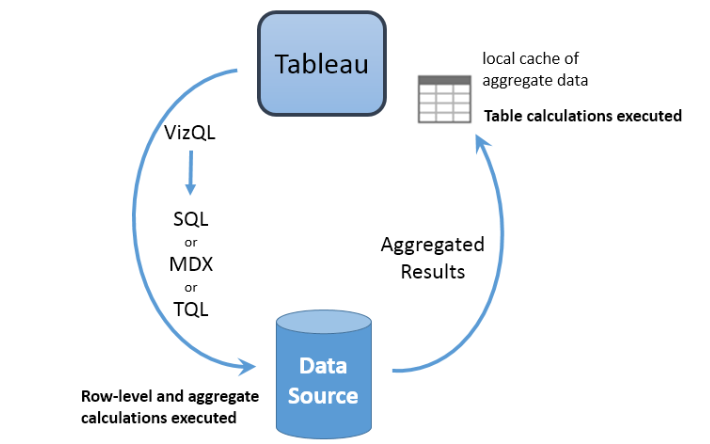
\includegraphics[width=0.8\linewidth]{Figures/TableCalculation.png}
    \end{center}
    \caption{Execution flow of a table calculation \protect\cite{LearningTableau}.}
    \label{fig:TableCalculation}
\end{figure}

Tableau gives the user the possibility to use a great variety of operations, but it's also possible to write a custom table calculation, such as:

\begin{itemize}
    \item Computing the running total.
    \item Computing time variance in both absolute values and percentage.
    \item Computing the moving and percentile average.
    \item Ranking or sorting according to specific functions.
\end{itemize}

\subsubsection{Analysis}

Another innovative feature present in Tableau is the possibility to make statistical analyses through mathematical models built-in or use algorithms written in \textbf{R, Python or MatLab} \cite{LearningTableau}. The main built-in models usable in Tableau are:

\begin{itemize}
    \item \textbf{Trend lines}: each trend line added to a chart represents a regression, which Tableau builds according to linear, logarithmic, exponential or polynomial models.
    \item \textbf{Forecasting}: in case of the visualization of a time series, it's possible to use the "exponential smoothing" method to compute future values according to an exponential function weighing current value and past values' average; Tableau can also recognize periodic patterns in time series.
    \item \textbf{Clustering}: Tableau uses K-Means algorithm to classify the data on the chosen variables and gives the user the possibility to change the value of K, that is the number of total clusters.
\end{itemize}

\section{Tableau Server}

\textbf{Tableau Server} is a server application used to contain data and metadata of sources and shared workbooks. Through an Access Control List based on accounts, Tableau server allows users to view, interact, download, share and edit a worksheet without the need install Tableau Desktop. Additionally, through the sharing of an already present data source, a user can create new worksheets without installing the correspondent drivers.

\subsection{Tableau Embedded}

Tableau Server offers the possibility to embed worksheets in a web application using Tableau JavaScript API, which allows for:

\begin{itemize}
    \item Viewing and interacting with the shared view.
    \item Loading and resizing the view dynamically.
    \item Download the view as a PDF or an image.
\end{itemize}

Corresponding user credentials would be required to view the shared charts and plots, but it's possible to use Tableau's \textit{Trusted Authentication} to authenticate the server hosting the application to allow all the web app user access to it.